%%%%%%%%%%%%%%%%%%%%%%%%%%%%%%%%%%%%%%%%%%  不使用 authblk 包制作标题  %%%%%%%%%%%%%%%%%%%%%%%%%%%%%%%%%%%%%%%%%%%%%%
%-------------------------------PPT Title-------------------------------------
\title{22-选讲专题:~机器学习方法简介}
%-----------------------------------------------------------------------------
%----------------------------Author & Date------------------------------------

%\author[\textrm{Jun\_Jiang}]{姜\;\;骏\inst{}} %[]{} (optional, use only with lots of authors)
%% - Give the names in the same order as the appear in the paper.
%% - Use the \inst{?} command only if the authors have different
%%   affiliation.
%\institute[BCC]{\inst{}%
\institute[Gain~Strong]{\inst{}%
%\vskip -20pt 北京市计算中心}
\vskip -20pt {\large 格致斯创~科技}}
\date[\today] % (optional, should be abbreviation of conference name)
{%	{\fontsize{6.2pt}{4.2pt}\selectfont{\textcolor{blue}{E-mail:~}\url{jiangjun@bcc.ac.cn}}}
\vskip 45 pt {\fontsize{8.2pt}{6.2pt}\selectfont{%清华大学\;\;物理系% 报告地点
	\vskip 5 pt \textrm{2023.04.22}}}
}

%% - Either use conference name or its abbreviation
%% - Not really information to the audience, more for people (including
%%   yourself) who are reading the slides onlin%%   yourself) who are reading the slides onlin%%   yourself) who are reading the slides onlineee
%%%%%%%%%%%%%%%%%%%%%%%%%%%%%%%%%%%%%%%%%%%%%%%%%%%%%%%%%%%%%%%%%%%%%%%%%%%%%%%%%%%%%%%%%%%%%%%%%%%%%%%%%%%%%%%%%%%%%

\subject{}
% This is only inserted into the PDF information catalog. Can be left
% out.
%\maketitle
\frame
{
%	\frametitle{\fontsize{9.5pt}{5.2pt}\selectfont{\textcolor{orange}{“高通量并发式材料计算算法与软件”年度检查}}}
\titlepage
}
%-----------------------------------------------------------------------------

%------------------------------------------------------------------------------列出全文 outline ---------------------------------------------------------------------------------
%\section*{}
%\frame[allowframebreaks]
%{
%  \frametitle{Outline}
%%  \frametitle{\textcolor{mycolor}{\secname}}
%  \tableofcontents%[current,currentsection,currentsubsection]
%}
%%在每个section之前列出全部Outline
%%类似的在每个subsection之前列出全部Outline是\AtBeginSubsection[]
%\AtBeginSection[]
%{
%  \frame<handout:0>%[allowframebreaks]
%  {
%    \frametitle{Outline}
%%全部Outline中,本部分加亮
%    \tableofcontents[current,currentsection]
%  }
%}

%-----------------------------------------------PPT main Body------------------------------------------------------------------------------------
\small
%\section{\rm{VASP~}软件中\rm{PAW~}计算的实现}
%\frame
%
%	\frametitle{\textrm{VASP}计算的特色}
%	相比于与普通的第一原理计算软件,\textrm{VASP}很好地平衡了计算效率和精度的问题,总的来说,\textrm{VASP}主要通过这几个特色保证了计算的高效能
%	\begin{itemize}
%	     \item 迭代与优化算法的多样性\\
%		     本质上电荷密度迭代 \textrm{\&\&} 体系总能量优化是相同的优化问题,采用了类似的算法\upcite{CMS6-15_1996,PRB54-11169_1996}:\\
%			\textcolor{blue}{\textrm{Pseudo-Newton、Conjugate-Gradient、Broyden~mix、damping-factor、RMM-DIIS}}
%	     \item 尽可能采用局域基(原子轨道基)函数:~\\
%		     \textcolor{blue}{\textrm{LREAL}}=\textcolor{red}{\textrm{.TRUE.}}\\
%			优化的投影函数也尽可能在实空间表示
%	     \item \textrm{PAW}原子数据集:\textcolor{blue}{优异的赝势}\upcite{PRB59-1758_1999}
%	\end{itemize}
%}
\frame
{
	\frametitle{科学研究的范式变更}
\begin{figure}[h!]
\vspace*{0.08in}
\centering
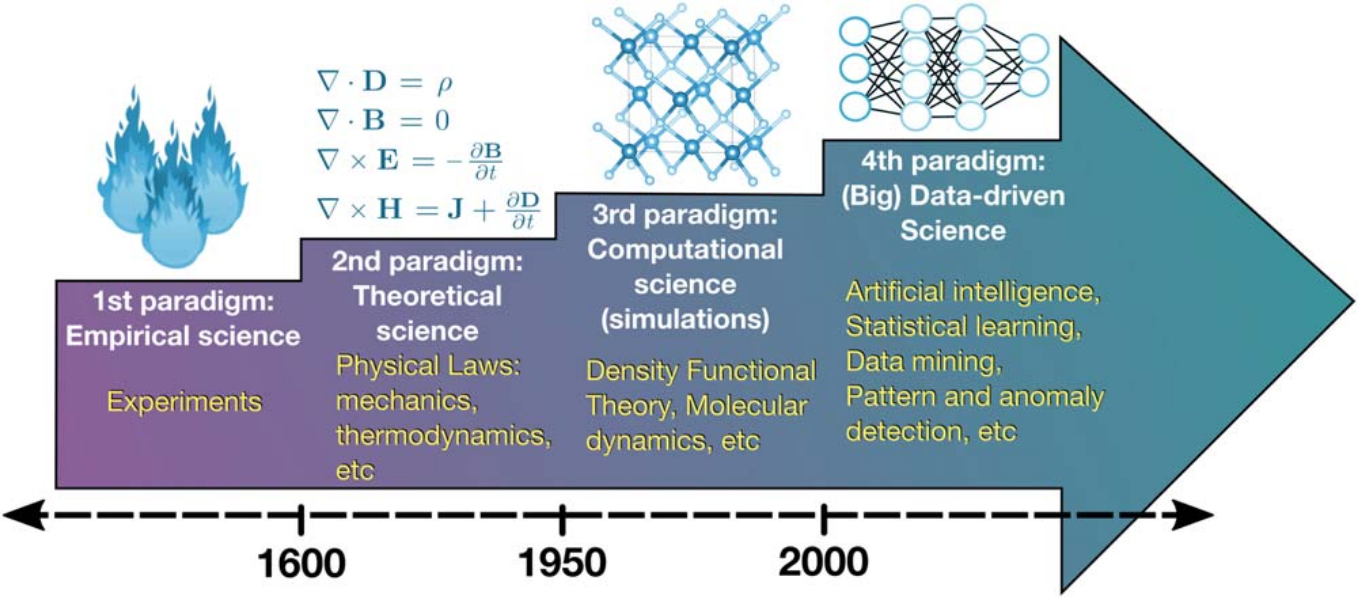
\includegraphics[height=2.00in,width=4.15in]{Figures/Four_Model_3.png}
%\caption{\tiny \textrm{Pseudopotential for metallic sodium, based on the empty core model and screened by the Thomas-Fermi dielectric function.}}%(与文献\cite{EPJB33-47_2003}图1对比)
\label{Four_Model}
\end{figure}
}

\frame
{
	\frametitle{机器学习\textrm{(Machine Learning, ML)}}
机器学习是自动完成数据分析并提取数据关系的一类方法的统称
\begin{figure}[h!]
\centering
\vspace*{-0.1in}
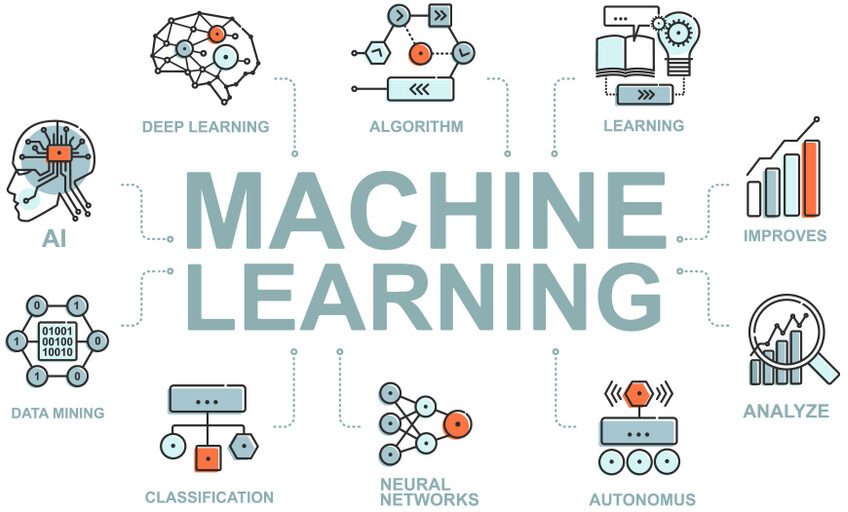
\includegraphics[height=2.3in,width=3.8in,viewport=0 0 630 390,clip]{Figures/Machine_Learning.jpg}
%\caption{\fontsize{7.2pt}{4.2pt}\selectfont{\textrm{人工智能与机器学习和深度学习的层次关系示意图.引自文献\cite{JPM2-032001_2019}}}}%
\label{Machine-Learning}
\end{figure}
\textcolor{blue}{用已知的数据关系预测未知数据或辅助不确定条件下的决策过程}
}

\frame
{
	\frametitle{人工智能\textrm{(Artificial Intelligence, AI)}与机器学习}
		获取材料完整物性数据的成本,无论是通过实验手段还是计算模拟,代价都是比较高
		\begin{itemize}
			\item 高通量第一原理计算自动流程和数据库解决了材料物性数据的获取问题%,但是并未给出现有材料数据基础上的物性优化的方案
			\item 利用数据挖掘技术,实现数据驱动的材料物性筛选、预测和提升的技术路线,有着特殊重要的意义
		\end{itemize}
	\vskip 8pt
	{\fontsize{8.2pt}{6.2pt}\selectfont{任何计算机模拟人类智能的算法都可以划归为人工智能,并非一定要应用机器学习算法,也包括决策树、知识库、计算机逻辑等算法
		\vskip 3pt
		{\fontsize{6.8pt}{4.2pt}\selectfont{\textcolor{blue}{人工智能广泛应用于金融、导航控制、语言处理、游戏竞技、计算机可视化和生物信息学等领域}}}
	\begin{itemize}
		\item 机器学习技术可以从大量数据中获得有价值的信息,尤其是面对高维复杂数据时,机器学习技术是确定数据间关系的有力的工具
	\item 机器学习领域的深度学习\textrm{(Deep Learning, DL)}是仿照生物神经网络\footnote{\fontsize{7.2pt}{6.2pt}\selectfont{神经网络结构意味着输入输出之间允许有多个类似神经的网络层}}结构为主要代表的一种示类学习
\end{itemize}}}
}

\frame
{
	\frametitle{人工智能和机器学习的层次关系}
	传统定义界定的机器学习,是指无须借助解析程序,直接依靠数据来提升任务处理的性能,自从\textrm{1950}年代统计学、计算科学与技术和神经科学的发展,机器学习的研究发展到了更广泛的人工智能领域%图\ref{AI-ML}表明了人工智能和机器学习的层次关系。
\begin{figure}[h!]
\centering
\vspace*{-0.1in}
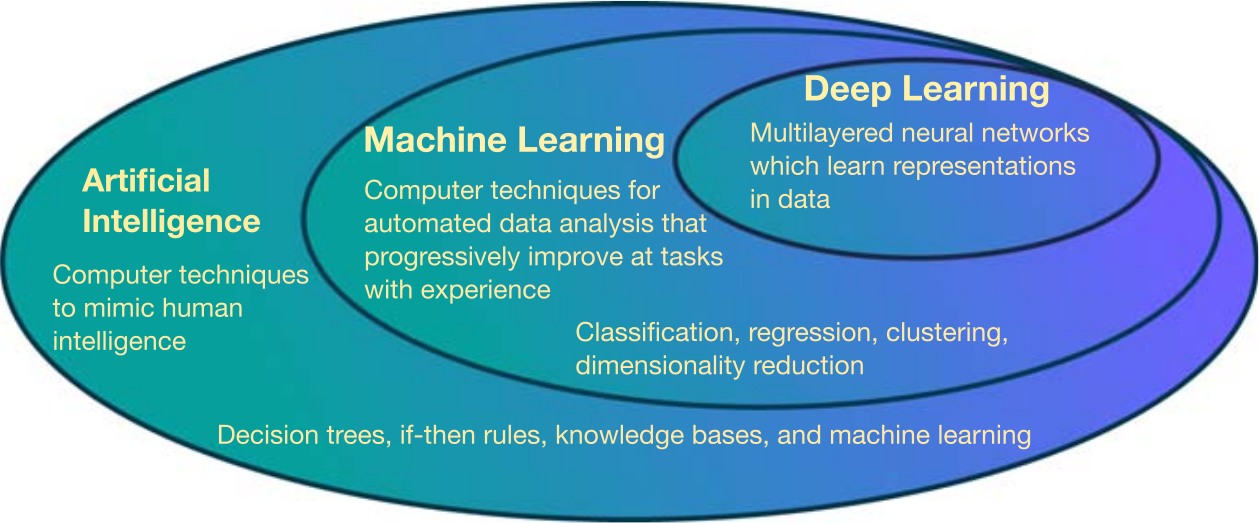
\includegraphics[height=1.9in,width=4.0in,viewport=0 0 1275 550,clip]{Figures/Hierarchical_description_AI_ML_DL.png}
\caption{\fontsize{6.2pt}{4.2pt}\selectfont{人工智能、机器学习和深度学习的层次关系示意图}}%
\label{AI-ML}
\end{figure}
}

\frame
{
	\frametitle{机器学习问题的一般形式与分类}
	\begin{itemize}
		\item 机器学习类问题的一般表示:
\vskip 5pt
对于给定的集合$\mathbf{X}$,可以预测或近似得到未知函数$y=f(\mathbf{X})$
\vskip 4pt
{\fontsize{6.2pt}{4.2pt}\selectfont{
	集合$\mathbf{X}$构成特征空间,集合中的每个元素$\mathbf{x}$称为特征向量(在材料类的机器学习中也称描述符)\\
	根据机器学习得到的近似函数$\hat{y}=\hat{f}(\mathbf{X})$,模型有能力预测训练数据之外的输出值}}
\vskip 5pt
	\textcolor{blue}{\fontsize{8.0pt}{4.2pt}\selectfont{机器学习的这种预测能力也称为模型的“泛化”\textrm{(generalization)}}}
\item 机器学习主要根据学习的特征分为无监督学习\textrm{(unsupervised learning)}和监督学习\textrm{(supervised learning)}
	\item 此外的机器学习问题还包括:~
\begin{itemize}
	\item 半监督学习,即大部分没有映射关系的数据和少量有映射关系的数据;
	\item 多任务和迁移学习,即将从相关问题习得的知识应用到数据极少的对象,提升模型的学习能力
	\item 强化学习,即没有输入输出,但会和环境不断交互,通过最大化环境的反馈,最终达到学习目标
\end{itemize}
	\end{itemize}
}

\frame
{
	\frametitle{无监督学习与监督学习}
\begin{itemize}
	\item 无监督学习是描述性质的,所有数据只有特征向量没有标签,但呈现出聚群的结构,每个相似的类型或特征的会聚集在一起\\
		如果没有标签的数据的组合是有限个,则称为聚类\textrm{(clustering)};~反之则称为密度估计\textrm{(density estimation)}\\
		另一种无监督学习是降维\textrm{(dimensionality reduction)},是对数据实施压缩,用少量输入变量代表数据,特别是高维数据,降维后有助于了解复杂数数据的检测模式
	\item 监督学习是预测性质的,是通过学习指定数量的输入输出间的函数映射\\
		如果输出函数$y_{\mathrm{i}}$表示类别的有限集合,则称为分类\textrm{classification}问题,模型可用来预测未知数据所属类型
		如果输出函数是实数,则称为回归\textrm{(regression)}问题\\
		模型用来预测未知输入数据对应的值输出值
\end{itemize}
}

